\section{Soft Error and Hard Error Resilience Design of ReRAM} \label{sec:arch}
A reliable cross-point ReRAM design should be resilient to both of the soft and hard errors. In our design, we proposed a detect-recognize-recover architecture to improve the reliability of the system. The error detection is realized by two-level ECC. The to recognize the error pattern, a multi-level sensing amplifier is applied. According to the error pattern, the recovery mechanisms are achieved either by boosted SET voltage or RESET current.

The proposed soft and hard error resilience design is shown in Fig.~\ref{fig:arch}. Firstly, a block-failure-table (BFT) is proposed to record the failure block and the failure behaviors of the block. As shown in Fig.~\ref{fig:arch}(b), the BFT is implemented as a content-addressable memory (CAM). Each entry in the table contains the physical address of the block, a HRS failure bit (HFB), and a LRS failure bit (LFB). Before every write operation, the BFT is checked to recognize if the hard errors has already appears at the accessed block. In order to mitigate the performance degradation and to guarantee the reliability, the BFT is implemented as a 1T1R structure. The number of the entries in the BFT directly affects the failures tolerance of the proposed architecture: although a larger BFT can record more failure blocks in the memory, the area and latency overhead will also increase significantly.


\begin{figure}[!t]
\centering
    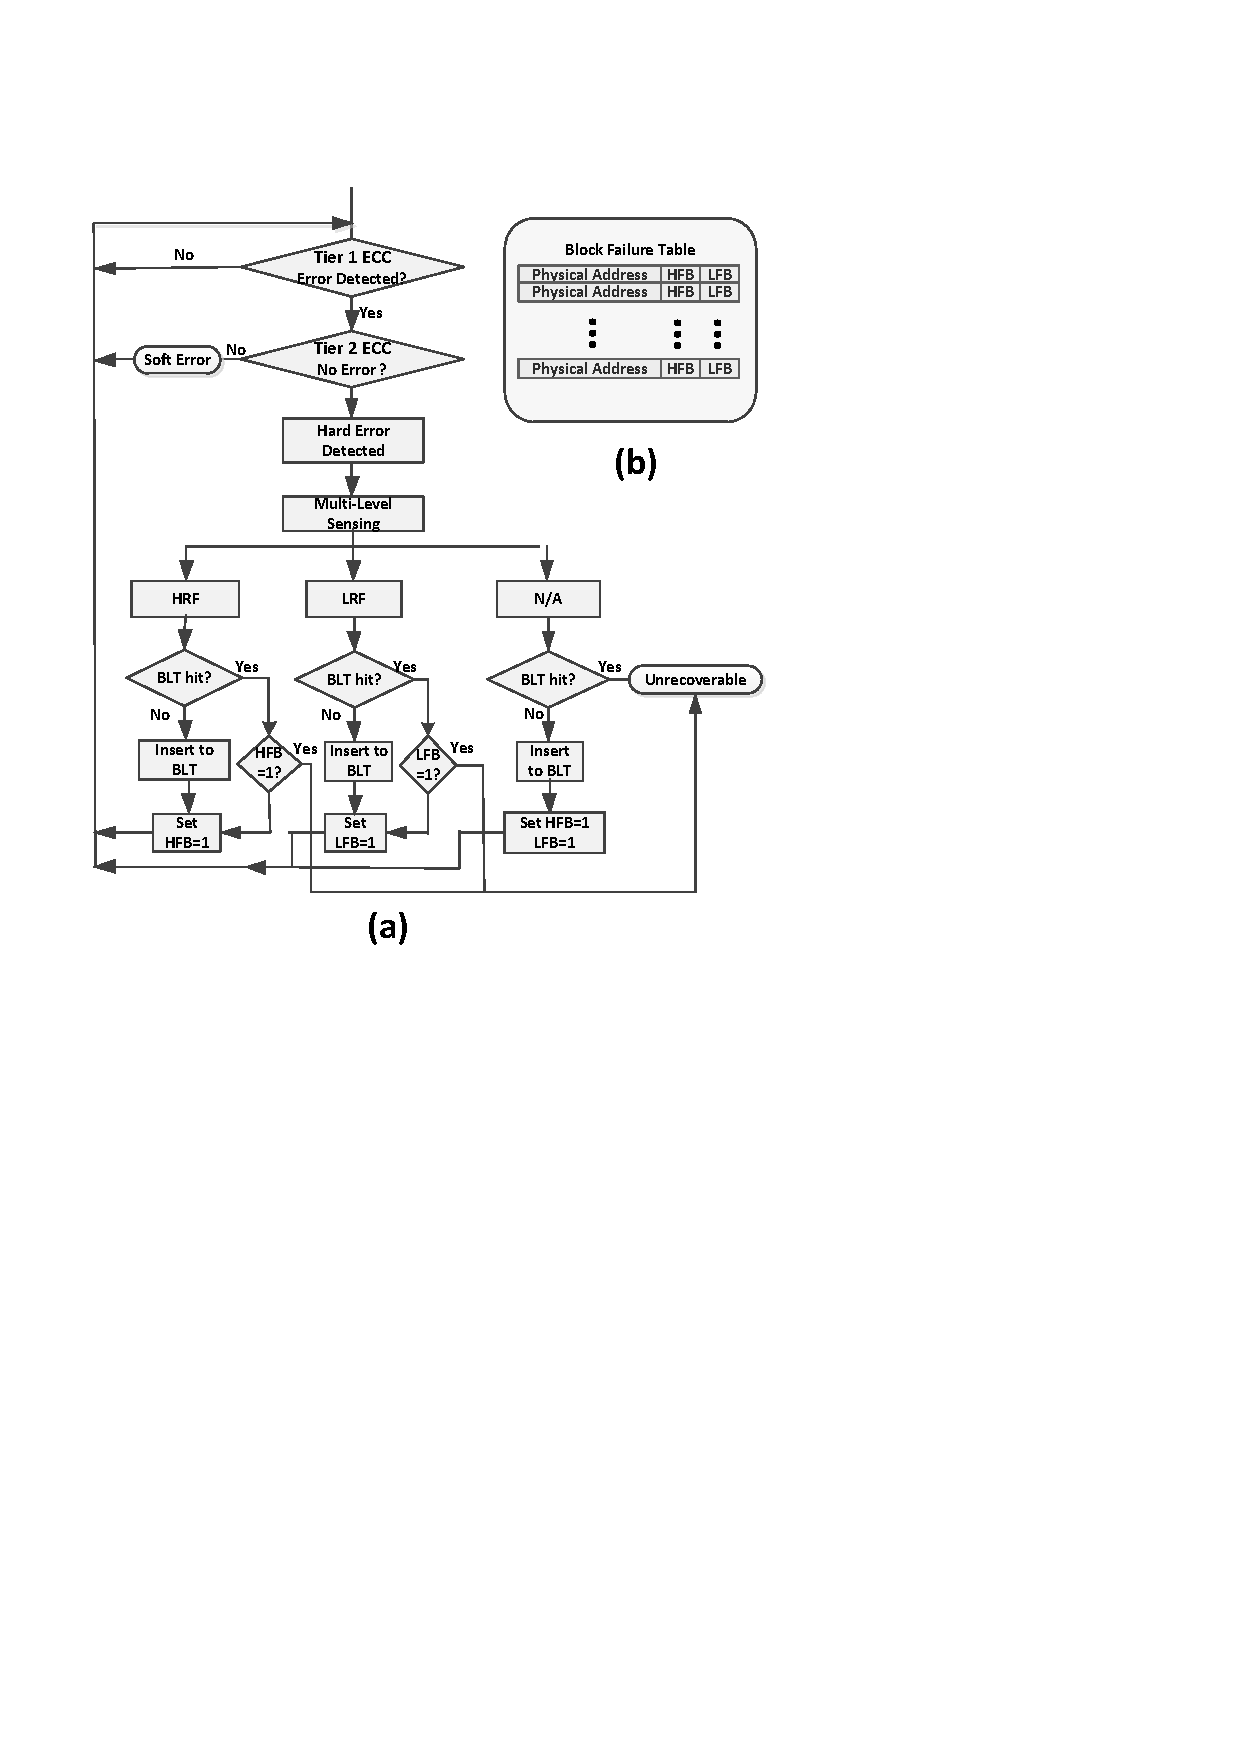
\includegraphics[width=3.4in]{./fig/arch.pdf}
\caption{(a) Soft and Hard Error Resilience Design. (b) BFT organization.}
\label{fig:arch}
\end{figure}

\begin{figure}[!t]
\centering
    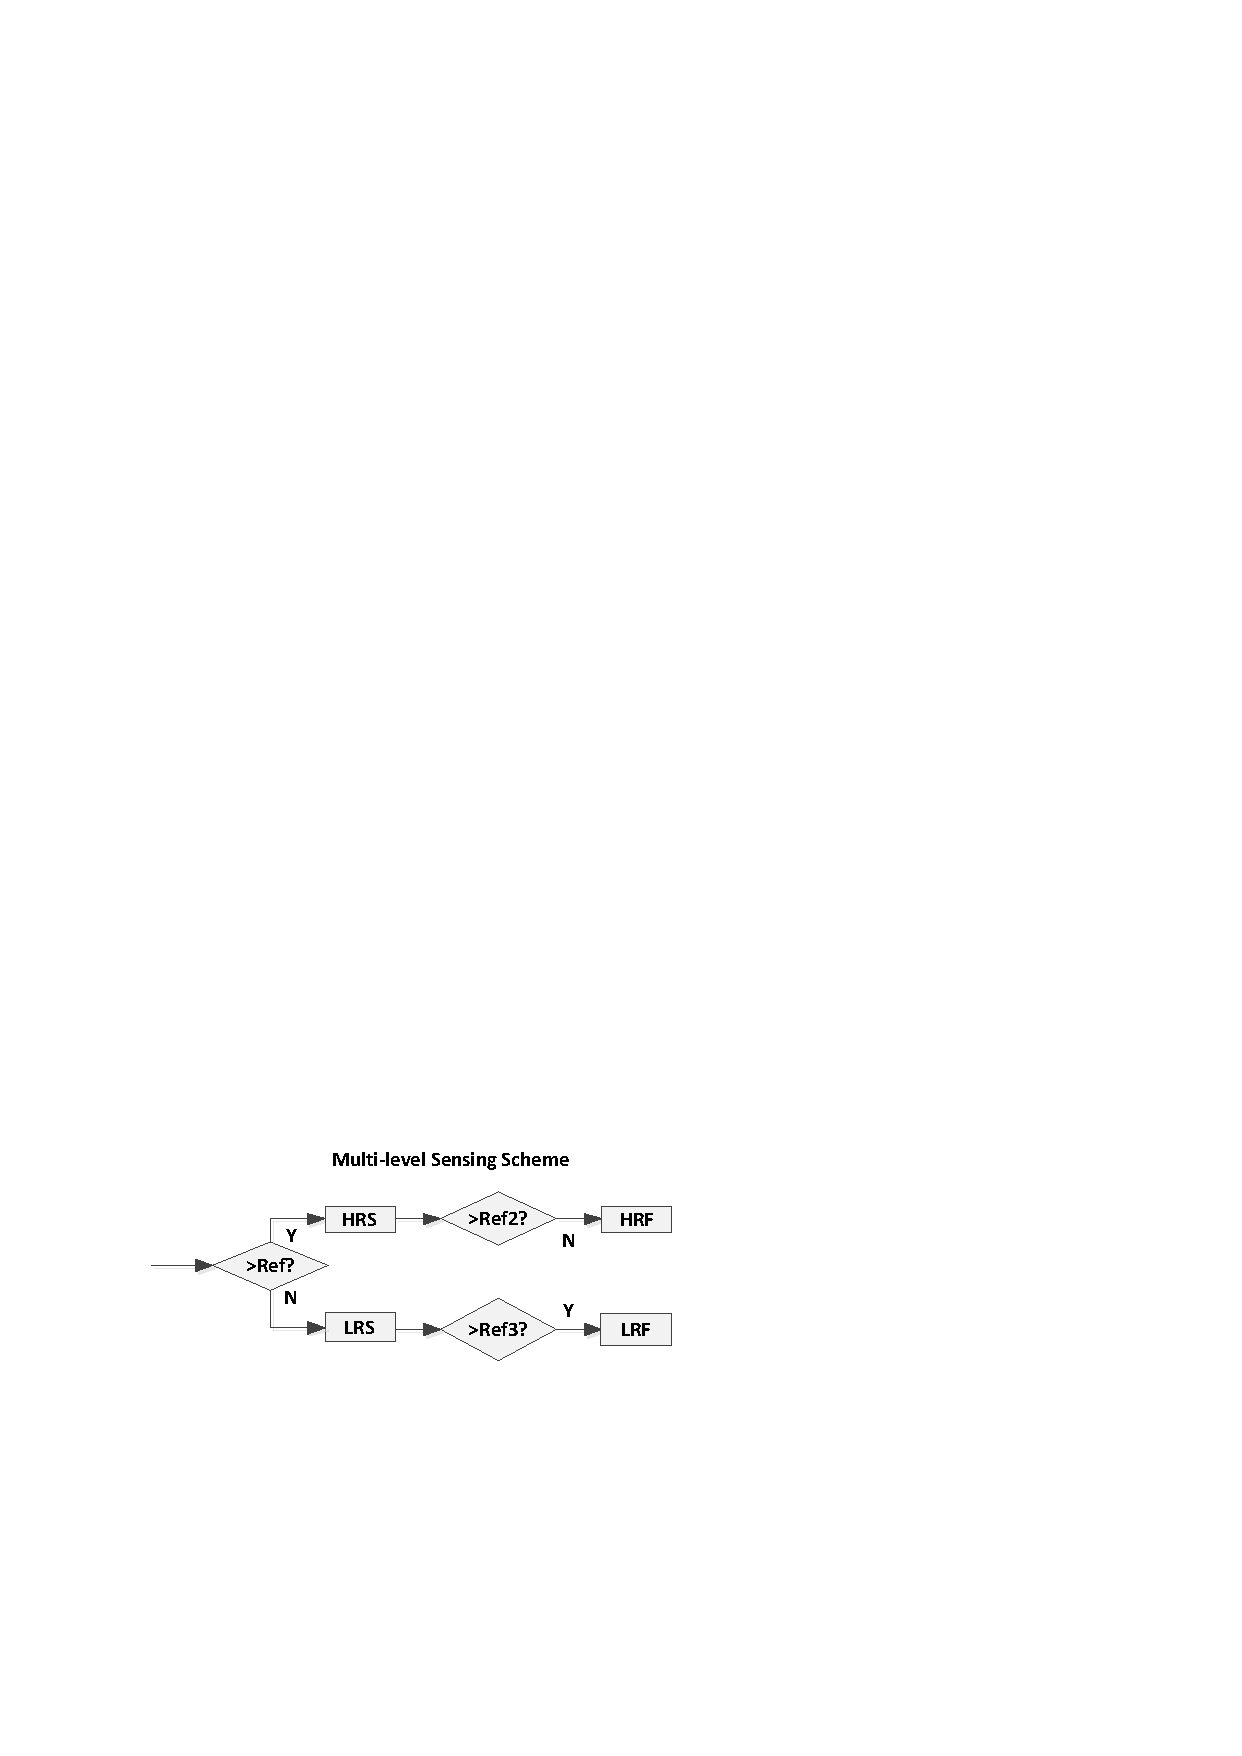
\includegraphics[width=3in]{./fig/sense.pdf}
\caption{Multi-level sensing scheme.}
\label{fig:sense}
\end{figure}

%In addition, the purpose of the proposed architecture is to detect the failure at a early stage and ensuring the system operate correctly at the same time.

The detection part is realized by two-level ECC: the first level ECC is a simple SEC-DED code, dealing with the soft error; the second level ECC is more complex with multi-bit correcting capability, which can detect and correct the errors results from the initial retention failure bits. If the first ECC level shows that no error detected, no further action is required. However, if the error is detected at the first level ECC, the data is sent to the second layer ECC. As soon as the multi-bit error is detected by level-2 ECC, the retention failure is confirmed. 

Simultaneously, the multi-level sensing is triggered to recognize the error pattern. As shown in Fig.~\ref{fig:sense} , the multi-level sensing can be used to distinguish the HRS failure and LRS failure. According to the output of multi-level sensing circuity, the corresponding bit (HFB or LFB) is updated. If the HFB or LFB is already been marked, the block is considered as a unrecoverable block and further replace action is required. Otherwise, the recover mechanisms will be performed during the following write operation to this block.

 

